%%%\documentclass[a4paper,10pt]{article}            %%% regular, using onecolumn,twocolumn params

\documentclass{../style/llncs}                   %%% for LNCS conf

%%%\documentclass[final]{siamltex}                  %%% for SIAM

%\documentclass[9.5pt,journal,final,finalsubmission,twocolumn]{../style/IEEEtran}%for IEEE trans
%\documentclass[12pt,journal,draftcls,letterpaper,onecolumn]{../style/IEEEtran} %for IEEE trans peer review

%%%\documentclass[acmtoms]{acmtrans2m}              %%% for ACM trans

%%%%\documentclass{../style/acm_proc_article-sp}    %%% for ACM proceedings
%%%% this solves the conflict between acm_proc_article-sp and algorithm2e conflict
%%%% like "too many }'s" error.
\makeatletter
\newif\if@restonecol
\makeatother
\let\algorithm\relax
\let\endalgorithm\relax
%%%%% end : conflict between acm_proc_article-sp and algorithm2e conflict


\usepackage{graphicx,subfigure,epsfig}
\usepackage{multirow}
\usepackage{latexsym,amssymb,amsmath,amsfonts}   %%amsthm
%%%%%%%%\usepackage{algorithmic, algorithm}
\usepackage[linesnumbered]{../style/algorithm2e}  %%% [linesnumbered,boxed]


%\newtheorem{theorem}{Theorem}[section]
%\newtheorem{conjecture}[theorem]{Conjecture}
%\newtheorem{corollary}[theorem]{Corollary}
%\newtheorem{proposition}[theorem]{Proposition}
%\newtheorem{lemma}[theorem]{Lemma}
%\newtheorem{definition}[theorem]{Definition}
%%%%%\newtheorem*{remark}{Remark} %% no numbering



%%% redefine proof environment
%%% Use this if no QED symbol at right corner in the last proof line !
\renewenvironment{proof}{\par\noindent{\em Proof.}}{\hspace*{\fill}$\square$\par}




\begin{document}
%\markboth{Hui Fang et al.}{Improving Piecewise-Linear Approximation by Relaxing on End Point Constraint}

\title{Multi-Stage Binary Code Obfuscation Using Improved Virtual Machine}

\author{Hui Fang\inst{1} \and Yongdong Wu\inst{1} \and Shuhong Wang\inst{2} \and Yin Huang\inst{2}  }
\institute{Institute for Infocomm Research\\
1 Fusionpolis Way, 21-01, Singapore 138632\\
\email{ \{hfang,wydong\}@i2r.a-star.edu.sg}\\
\and Sumavision Soft Tech Co., Ltd.\\
15 Kaituo Road, Shangdi District, Beijing, 100085, China\\
\email{\{wangshuhong,huangyin\}@sumavision.com} 
}







%%%\thanks{H. Fang and Y. Wu are with the Singapore-MIT Alliance program, Nanyang Technological University, N4-02b-40, 65 Nanyang Drive, Singapore 637460 e-mail: fang0025@ntu.edu.sg, hsu@ntu.edu.sg}





%\numberofauthors{3}
%\author{
%\alignauthor Hui Fang\\
%       \affaddr{Nanyang Technological University}\\
%       \affaddr{65 Nanyang Drive, Singapore 637460}\\
%       \email{fang0025@ntu.edu.sg}
%\alignauthor Wen-Jing Hsu\\
%       \affaddr{Nanyang Technological University}\\
%       \affaddr{N4-02b-40, 65 Nanyang Drive, Singapore 637460}\\
%       \email{hsu@pmail.ntu.edu.sg}
%\alignauthor Larry Rudolph\\
%       \affaddr{VMware Inc.}\\
%       \affaddr{5 Cambridge Center, Cambridge, MA, USA}\\
%       \email{rudolph@vmware.com}
%}

%%%\date{}
\maketitle

\begin{abstract}
A software obfuscator transforms a program into another executable one with the same functionality but unreadable code implementation. This paper presents an algorithm of multi-stage software obfuscation method using improved virtual machine techniques. The key idea is to iteratively obfuscate a program for many times in using different interpretations. An improved virtual machine (VM) core is appended to the protected program for byte-code interpretation. Adversaries will need to crack all intermediate results in order to figure out the structure of original code. Compared with existing obfuscators, our new obfuscator generates the protected code which performs more efficiently, and enjoys proven higher level security. 
\end{abstract}


%\begin{keywords} software security, code obfuscation, virtual machine.\end{keywords}




%\begin{AMS} 15A15, 15A09, 15A23  \end{AMS}
%\pagestyle{myheadings}
%\thispagestyle{plain}
%\markboth{}{Improving Piecewise-Linear Approximation by Relaxing on End Point Constraint}
%Hui Fang et al.



%\category{G.1}{Mathematics of Computing}{Numerical Analysis}
%\category{I.3.5}{Computing Methodologies}{Computer Graphics}[Computational Geometry and Object Modeling]
%\terms{Algorithms}
%\keywords{tracking, particle filter, activity map, personal positioning}

%\setcounter{page}{1}

%\begin{bottomstuff}
%Author's address: L. Lamport, System Research Center,
%Digital Equipment Corporation, 130 Lytton Ave., Palo Alto, CA
%94301.\newline
%Start of a second footnote ...
%\end{bottomstuff}





\section{Introduction}

Software obfuscation refers to transformations on the code which
becomes hard to understand while preserving all functionalities.
It plays an importance role in protecting confidential data and algorithms
from reverse engineering or virus modification
\cite{collberg97,collberg02,madou06a,cappaert08}.
Ideally, an adversary possessing a well-obfuscated program
should be only able to learn program input/output like a black-box access.
Due to this, software obfuscation has received many research
interests for the last ten years
\cite{barak01,schwarz02,ogiso03,oorschot03,lynn04,madou06b,anckaert07,beaucamps07,collberg09}.


%%%% problem statement, challenges
The challenge in software obfuscation lies in
whether or not guaranteed security and fair performance
can be provided for obfuscated binary code.
Specifically, code security implies resistance to
static analysis and even dynamic analysis, and code efficiency
implies that the obfuscated code should not run much slower
than the original code.
Up to now, some practical metrics for software obfuscation have been proposed
in the literature \cite{mit03,lynn04,madou06a,naeem07,anckaert07,ceccato09}.
Meanwhile, obfuscation on Turing machine programs with formal definitions
has been researched intensively as well
\cite{barak01,ogiso03,goldweisser05,wee05,canetti08,bitansky10,hohenberger10,canetti10}.
Unfortunately most practical obfuscation techniques
lack a well-founded theoretical base, and thus it is unclear
how effectively they perform.
We take consideration of both practical and theoretical obfuscation metrics,
and design our obfuscation algorithm align to theoretical definitions in principle.


%%%% main contributions
We address the challenge by presenting an algorithm of multi-stage software obfuscation using
improved virtual machine.
The key idea is to obfuscate a software for many times while each time
applying different interpretations in order to improve security.
To fulfil the purpose, an improved virtual machine core
responsible for byte-code interpretation is appended to the protected software.
Under this design, an adversary must crack all intermediate results in order to figure out
the structure of original code.
Compared with existing obfuscators,
our new obfuscator creates obfuscated code which performances more efficiently,
and enjoys a higher security level.


%%%%% section organization
The paper is organized as follows.
Section \ref{section_sw_obfuscation} introduces the related work on
software obfuscation and virtual machine.
Section \ref{section_approach} describes our approach in two steps:
block-to-byte virtual machine and multi-stage code obfuscation.
Section \ref{section_analysis} analyzes the security of our new
software obfuscation algorithm.
Section \ref{section_expr} provides experimental results.
Finally, Section \ref{section_conclusion} draws a conclusion.




\section{Related Work} \label{section_sw_obfuscation}


Most existing obfuscation techniques on binary code fall into three categories:
\begin{itemize}
  \item data transformation, such as name renaming and string encryption.
  \item instruction transformation, which replaces binary instructions using a
  library of equivalent instructions.
  \item control flow transformation, which transforms the graph structure of program control flow.
\end{itemize}

Data transformation does not alter program controls. Even the encrypted data
will have to be decrypted inside the program for use. The code for
decryption again faces the attack from reverse engineering.
Therefore data obfuscation is usually applied together with
other complicated obfuscation techniques to increase security
\cite{monden04,hohenberger07,sivadasan09}.

Control flow transformation is relatively complicated
\cite{wang01,jhala05,ge05,preda06,abadi10}.
Typically a control flow flattening method puts all basic blocks into a single switch
statement which maintains whole control flow.
It obfuscates the order
in which the computations are carried out,
in order to stand against static analysis.
However, constant propagation on
the switch variable will expose the next block to be executed.
Besides, one large switch statement will generate many jumps which
decreases program performance.
Opaque predicates are boolean expressions whose values are known to the
obfuscator but difficult for adversary to deduce. Junk codes are usually inserted
into the dead path of an opaque predicate.
However, for the same reason as above,
there still exists risk that an adversary may figure out the value of an
opaque predicate by static analysis.

Instruction transformation refers to replacement of protected binary instruction
with a block of instructions which is functionally equivalent
\cite{linn03,kanzaki04,madou05,popov07,rolles09}.
The introduced blocks representing native instruction are written as byte-codes
into the program. Those byte-codes are often maintained by a virtual machine
integrated with the obfuscated program.
In practice, instruction transformation works well against static analysis
except for runtime disassembly.
However, little theoretical work has been carried out to show
guarantee on its security and performance on obfuscated software.


%%%%% turn to VM
Virtual machine (VM) based obfuscation recently becomes popular
for software obfuscation,
and it is probably the most sophisticated in the literature
\cite{smith05,sharif09,rolles09}.
It usually integrates several obfuscation techniques including data
permutation, instruction institution, and control flow transformation.
As a result, VM obfuscation is fairly good against dynamic analysis
in practice \cite{vmprotect,oreans,x86virtualizer}.
We observe the common way how VM obfuscator works, and summarize
a general code structure for the program before and after obfuscation
as shown in Figure \ref{fig_obf_virtualizer}.
Generally speaking, a VM section will be appended to the original program,
and the protected binary code will be transformed to byte-code,
which is interpreted by a VM core. Finally, the entry point of the program
will be redirected into VM code.
To fulfil the byte-code fetching, VM core still
needs to save all registers and flags in its own context,
and to restore upon exiting byte-code interpretation.

\begin{figure}  \centering
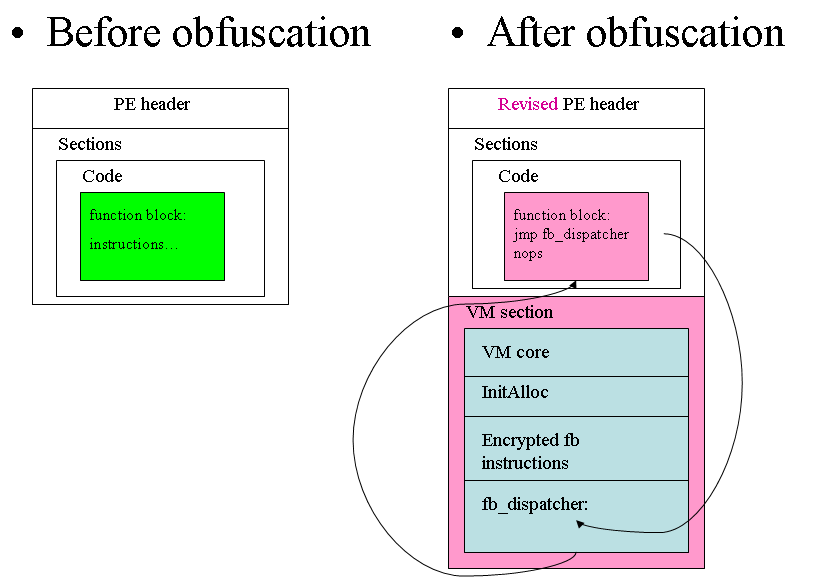
\includegraphics[width=0.7\columnwidth]{./figure/fig_obf_virtualizer}
\caption{Virtual machine based obfuscation.}
\label{fig_obf_virtualizer}
\end{figure}

%%%% VM weakness
Classical VM obfuscators suffer two drawbacks.
Firstly, they generate obfuscated software which runs
much slower than the original one. It is largely
because of byte-code interpretation working style \cite{oreans,vmprotect}.
Secondly, the security of VM obfuscated program
relies merely on an uncustomized VM core integrated with program
rather than each individual program.
VM does not restore byte-codes to original
instructions any more.
Therefore success of attacking obfuscated program requires two steps:
understanding VM code, and decoding mapping
between binary instructions and byte-codes.
One round VM obfuscation will output relatively intelligible mapping,
which allows an adversary to perform instruction level
analysis, and further to reconstruct the structure of original
software \cite{sharif09,rolles09}.


The existing works are promising under certain situations.
However, the danger of software cracking is always
changing and increasing \cite{udupa05,madou06b}.
Therefore we propose a new approach on software obfuscation
in next section, introducing a more light-weighted obfuscator
which generates harder understanding codes.



\section{Our Approach} \label{section_approach}


In this section we firstly introduce the concept of black box security,
then present new design of block-to-byte virtual machine,
and describe a framework of multi-stage code obfuscation
based on improved virtual machine.

A program obfuscator is often regarded as a processor on
computer programs, which outputs a new program of the same functionality
but with unreadable code structure \cite{ogiso03,collberg09}.
More precisely, a program obfuscator $O$ is theoretically defined to be
a probabilistic Turing machine or Boolean circuit,
which satisfies three requirements \cite{barak01}:
\begin{itemize}
  \item (Functionality Equivalence) For every TM/circuit $P$ and for every input $x: P(x) = O(P)(x)$.

  \item (Polynomial Slowdown) There exists a polynomial $q(.)$ such that for every TM/circuit $P$, $|O(P)| \le q(|P|)$.
TMs are additionally required that for every input $x$, if $P$ halts after $t$ steps on $x$ then $O(P)$ halts within $q(t)$ steps on $x$.

  \item (Virtual Black Box) For any PPT $A$, there is a PPT oracle machine $S$ and a negligible
   function $negl(.)$ such that for all TM/circuit $P$:
$| Pr[A(O(P))=1] - Pr[S^P(1^{|P|})=1] |  <  negl(|P|)$.

\end{itemize}


Although Barak et al. \cite{barak01} further proved that this kind of universal black box
obfuscator does not exist, the theoretical concept
is still useful in evaluating performance of code obfuscators.
In other words, a good obfuscator shall as best as possible promise three properties:
function equivalence, code efficiency, and black box security.
In light of these requirements we present our customized VM obfuscator below.



\subsection{Block-to-Byte Virtual Machine}


The core of a virtual machine(VM) is a \emph{dispatcher} which transforms byte-code
to an implementation of binary instructions.
To adapt to the purpose of program obfuscation,
virtual machine must have \emph{byte-codes} populated in and contain
the \emph{implementations} of all byte-codes
for the program to protect. Specifically, a virtual machine will fetch byte-code
one by one, position the target address in its \emph{jump table}, and give
control to the instruction in that address.
So a complete virtual machine to be appended to the
obfuscated program will be
\[
    V:= \{ Bytecodes, Impl, Jmptable, Dispatcher
    \}.
\]

Classical VM obfuscator will map each binary instruction to a byte-code,
together with its implementation (as described in Algorithm \ref{algo_obf_ord_vm}).
We revise the design and present a block-to-byte VM obfuscation algorithm,
as shown in Algorithm \ref{algo_obf_b2b_vm}. The major difference lies in that
a control flow graph (CFG) of the program is set up in prior, and then the
obfuscator maps each basic block of the graph into a byte-code based on which
the obfuscation is carried out.

\begin{algorithm}
\caption{Classical VM based obfuscation.}
\label{algo_obf_ord_vm}
 \KwIn{Original program $P$.}
 \KwOut{Obfuscated program $Q$.}
  create a virtual machine $V$ for $P$\;
  $V.Impl =\{\}$\;
  $V.Bytecodes =\{\}$\;
  \For {binary instruction $b \in P$ }
  {
     translate $b$ into byte-code $B$ with implementation $I(b)$\;
     $b=$ instruction ``jump to $V$''\;
     $I(b)$'s last instruction = ``jump to next to $b$''\;
     $V.Jmptable[B] = I(b)$\;
     $V.Bytecodes += B$\;
     $V.Impl += I(b)$\;
  }
  output $P+V$\;
\end{algorithm}

\begin{algorithm}
\caption{Block-to-byte VM based obfuscation.}
\label{algo_obf_b2b_vm}
 \KwIn{Original program $P$.}
 \KwOut{Obfuscated program $Q$.}
  construct control flow graph, $CFG(G)$\;
  create a virtual machine $V$ for $P$\;
  $V.Impl =\{\}$\;
  $V.Bytecodes =\{\}$\;
  \For { block $BL \in CFG(P)$ }
  {
     translate $BL$ into byte-code $B$ with $I(BL)=\sum_{b\in BL}I(b)$\;
     $BL$'s first instruction = ``jump to $V$''\;
     $I(BL)$'s last instruction = ``jump to last of $BL$''\;
     $V.Jmptable[B] = I(BL)$\;
     $V.Bytecodes += B$\;
     $V.Impl += I(BL)$\;
  }
  output $P+V$\;
\end{algorithm}

Figure \ref{fig_obf_bytecode} shows the format for binary
instructions and VM byte-codes respectively. It also gives
an example how a binary instruction was transformed into byte-code
together with an implementation.

\begin{figure}  \centering
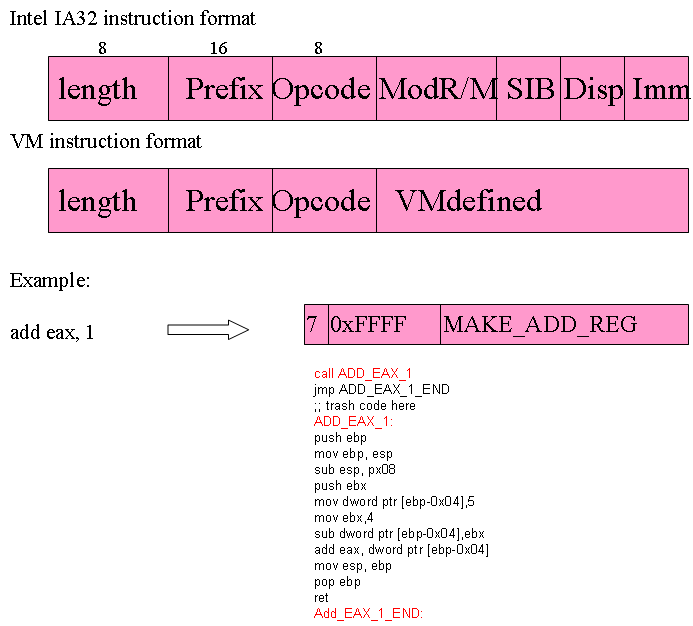
\includegraphics[width=0.7\columnwidth]{./figure/fig_obf_bytecode}
\caption{Format of VM byte-code instruction and an example of implementation.}
\label{fig_obf_bytecode}
\end{figure}

VM dispatcher works on stack based style:
it saves registers for native code and create own VM stack.
The return value of last execution for each byte-code was saved in VM registers
(\emph{var\_RegEip} and \emph{var\_RegDI} in Figure \ref{fig_obf_dispatcher})
for next byte-code execution.
VM dispatcher then obtains the target address by searching a jump table using byte-code
as index.
Target address is the location that current instruction will transfer to.
VM obfuscator retrieves all target addresses of the original program in
four different ways:
for direct jump, target address is specified in the original instruction;
for conditional jump, there are two target addresses with a predicate;
for call instruction, one target address is set for called function, and
another one for return address;
and for return instruction, target address is stored on the stack.


\begin{figure}  \centering
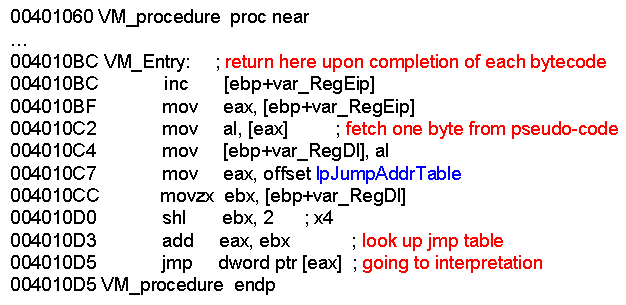
\includegraphics[width=0.7\columnwidth]{./figure/fig_obf_dispatcher}
\caption{VM byte-codes are executed by a dispatcher.}
\label{fig_obf_dispatcher}
\end{figure}




\subsection{Multi-Staged Code Obfuscation}

In this section we extend the technique of block-to-byte virtual machine to
a multi-stage obfuscation.
The idea of multi-stage obfuscation algorithm is described as follows.
Given an original program $P$, we choose a random number $n$ to be
the number of obfuscation stages, a one-way function $f$, and
an obfuscation function $Obf$. Then we calculate multiple copies
$\{P_0, P_1,...,P_n\}$ of
the program together with the keys $\{K_0,K_1,...,K_n\}$
for each obfuscation stage, as shown in Figure \ref{fig_obf_algo}.

We iteratively obfuscate program $P$ for $n$ times.
The obfuscation key $K_i$ is generated from each intermediate program
$P_i$ of the previous obfuscation stage, and $K_i$ is again applied to $P_i$ to
compute $P_{i+1}$.

\begin{eqnarray*}
  K_i     &=& f(P_i), \\
  P_{i+1} &=& Obf(P_i, K_i).
\end{eqnarray*}

The function $f$ maps any program into a key in binary string, satisfying
that: $f$ must have one-way hardness, and the output key can characterize
the program. The examples of this type of function include: MD5 hash value
of program where the program is feed as data, or the number of nodes in program's
control flow graph.

\begin{figure}  \centering
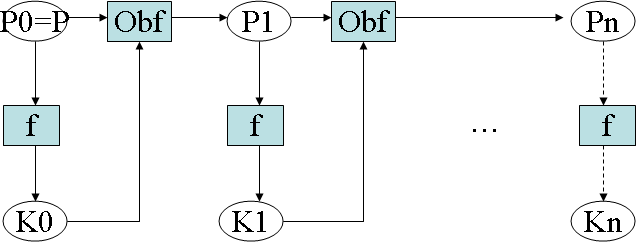
\includegraphics[width=0.7\columnwidth]{./figure/fig_obf_algo}
\caption{The multi-stage obfuscation algorithm. $P_n$ is output.}
\label{fig_obf_algo}
\end{figure}

The obfuscation of program requires to hide program's data and/or control flow while
preserving all the functionalities. In other words, each copy $P_i$ of the program must
be executable and function normally. Our idea is to extract all $jmp/jcc/call$ points
of $P$, and transform such information into a jump table. Then the jump table is obfuscated
given a particular $K$ and some dummy codes.
Original program $P$ is thus modified accordingly to
jump table to preserve correct control.
In other words, a separate hidden jump table will take control over program's running.
Adversaries need to crack all intermediate obfuscated programs in order to recover original
code's control flow.
%%%%%A formal description is summarized in Algorithm \ref{algo_obf_multistage}.

%%%\begin{algorithm}
%%%\caption{Multi-stage program obfuscation.}
%%%\label{algo_obf_multistage}
%%% \KwIn{Original program $P$, and the number $n$ of obfuscation stages.}
%%% \KwOut{Obfuscated program $P_n$.}
%%%  $P_0=P$\;
%%%  $K_0=f(P_0)$\;
%%%  \For { $i =1,2,...,n$ }
%%%  {
%%%     construct the $CFG(P_{i-1})$\;
%%%     $P_i = Obf(P_{i-1}, K_{i-1})$\;
%%%     $K_i= f(P_i)$ \;
%%%  }
%%%  output $P_n$ only \;
%%%\end{algorithm}





For intra-block instructions or a single instruction,
we use a revised tree structure to describe the whole process of multi-stage obfuscation.
In this tree structure,
each node represents a list of binary instructions (as shown in example of Figure \ref{fig_obf_polymor}).
The root node $x_1$ refers to only one binary instruction,
denoted by a circle. It links to its three children, $V_1, V_2, V_3$, which are different
implementations of $x_1$. The children are called byte-codes, drawn in rectangles.
Each byte-code, e.g. $V_1$, contains
a list of binary instructions, e.g. $y_1 \rightarrow y_2 \rightarrow y_3$.
In Stage-1 obfuscation, $x_1$ is assumed to be
mapped into byte-code $V_2$; further in Stage-2, $y_4$ and $y_5$ of $V_2$
are mapped into $V_5$ and
$V_6$ respectively.
The path selection from an earlier stage to next stage is determined by
$K_i$. In the example case, a formal induction of resulted code would be
\begin{eqnarray*}
x_1 &=& V_2  \\
    &=& y_4 \rightarrow y_5  \\
    &=& V_5 \rightarrow V_6  \\
    &=& (z_3 \rightarrow z_4 \rightarrow z_5) \rightarrow (z_6 \rightarrow z_7) \\
    &=& z_3 \rightarrow z_4 \rightarrow z_5 \rightarrow z_6 \rightarrow z_7.
\end{eqnarray*}




%%%%% Figure
\begin{figure}  \centering
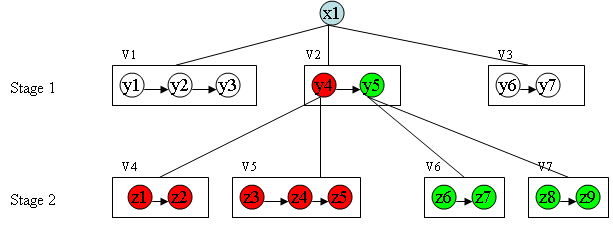
\includegraphics[width=0.7\columnwidth]{./figure/fig_obf_polymor}
\caption{Tree structure used in multi-stage obfuscation.}
\label{fig_obf_polymor}
\end{figure}








\section{Security Analysis} \label{section_analysis}


This section analyzes the security of multi-stage obfuscated program
in two aspects: code efficiency and black box security.
Specifically we strengthen the black box security by introducing
code polymorphism during multi-stage obfuscation,
and improve the code efficiency by removing unnecessary jump
instructions during block-to-byte VM obfuscation.

\subsection{Multi-Stage Polymorphism}

Polymorphism refers to that one binary instruction could have many byte-code
interpretation with equivalent function. It is often used in code obfuscation
to improve the difficulty in reversing program to original status.

When one instruction was obfuscated over twice,
the mapping relationships from binary to byte codes become unrecognizable,
due to many possible instruction combinations.
Given an instruction sequence $z_3 \rightarrow z_4 \rightarrow z_5 \rightarrow z_6 \rightarrow z_7$,
an adversary needs to separate them into byte-codes to understand the original program structure.
In other words, one cannot easily
split a sequence of instructions into correct $\{V_5, V_6\}$,
and further obtain byte code $V_2$ which refers to $x$ in first stage.
Generally speaking, the fan-out width $W$ of each binary node and the block size $L$ of byte-code
node for each stage
determine the obfuscation complexity.
In addition, the number $n$ of stages is randomly chosen to control the complexity.
The complexity of guessing increases exponentially with the number of stages.
In this sense, multi-stage polymorphism makes the obfuscation of software more secure
than the one obfuscated by single VM obfuscation.
This claim is proved in Theorem \ref{theorem_poly}.




\begin{theorem} \label{theorem_poly}
An  $n$-stage polymorphism tree provides $C(n)$ possible implementations
for root node given constant $W$ and $L$, where $C(n) = W^{L^{n-1} +...+L+1}$.
\end{theorem}
\begin{proof}
Use mathematical induction. When $n=1$, root node links to $W$ children which are
all available choices. So $C(1)= W$ satisfies the equation.
Assume $C(k) = W^{L^{k-1} +...+L+1}$, and consider the case when $n = k +1$.
Firstly we notice that the number of choices owned by a binary component of each stage-1 node is
$C(k)$. Since each node has $L$ components, there will be $C(k)^L$ choices for solution
passing through this node. Secondly we notice that the root node can choose path from its
$W$ children. So the total possible paths will be
\begin{eqnarray*}
C(k+1) &=& W* C(k)^L   \\
       &=& W*(W^{L^{k-1} +...+L+1})^L  \\
       &=& W*( W^{L^k+...+L^2+L} )  \\
       &=& W^{L^k+...+L^2+L+1},
\end{eqnarray*}
which completes the proof.
\end{proof}



\subsection{Improved Execution Efficiency}

The classical VM obfuscator transforms protected code into
byte-codes. The resulted obfuscated program then interprets byte-codes
sequentially, and runs the implementation of byte-codes accordingly.
However, the program control will be unconditionally switched to VM dispatcher
every time when one byte-code interpretation is completed.
The number of $jmp$s inserted for byte-code interpretation is proportional
to the number of binary instructions.
It is well known that the jump operations block the instruction streamline for execution.


In contrast, our block-to-byte VM obfuscation chooses a ``basic block'' to execute
before jumping back to VM dispatcher. There will be no new $jmp/jcc/call$ instruction
inserted inside one basic block. The obfuscated program only needs to interpret
bytes representing basic blocks and follows the original control flow of the
program. So the number of $jmp$s inserted for byte-code interpretation
is only proportional to the number of nodes in program control flow graph.
By interpreting a block of instructions into only one byte-code,
our multi-stage VM obfuscator is able to reduce those unnecessary jumps during
code obfuscation.


The number of $jmp$ instructions in the program plays a heavy part in
slowing down the program execution time. Given an average block size $L$ of
control flow graph of the program, our block-to-byte VM obfuscator will generate
only $\frac{1}{L}$ the number of $jmp$ instructions by the classical one.




\section{Experiments} \label{section_expr}

The testing experiment on our multi-stage VM obfuscation module
was carried out on WinXP 2.4GHz CPU and 1G RAM platform.
A demo of obfuscation out is given in Appendix \ref{section_appendix}.
Three parameters are take into consideration: structure of control
flow graph, program size, and running time of obfuscated program.
We adopt IDApro \cite{idadebugger}, a disassembly tool
to facilitate view on IA-32 executables. VMprotect \cite{vmprotect},
a popular VM obfuscation software, was chosen for empirical comparison.


\subsection{Control Flow Graph}

The complexity of a program's control flow graph reflects
program intelligibility to certain extent. We capture
the number of nodes and edges in graph as an indicator
of graph complexity. Accordingly, the \emph{obfuscation level}
is hereafter defined as the ratio of number of nodes
or edges in CFG before and after obfuscation.
Table \ref{tab_obf_control_flow_graph} presents the obfuscation
level for programs using multi-stage VM obfuscation.
It implies that the control flow graph becomes interleaved which
leads to high obfuscation level of program.


\begin{table}  \centering
\caption{The number of nodes and edges of control flow graph before and after obfuscation. } \label{tab_obf_control_flow_graph}
\small % change the font size
\begin{tabular}{ |l|c|c|c|c|c|c| }
\hline
\multirow{2}{*}{Program} & \multicolumn{2}{|c|}{Original} & \multicolumn{2}{|c|}{Obfuscated}  & \multicolumn{2}{|c|}{Obfuscation Level}    \\
\cline{2-7} & \#nodes,$N$ & \#edges,$E$ & \#nodes,$N_2$ & \#edges,$E_2$ & $N_2/N$ & $E_2/E$ \\
\hline \hline
 md5     &  437 & 164  &  581    &  353  & 1.33  & 2.15 \\
 calc    &  458 & 175  &  746    &  308  & 1.63  & 1.76 \\
 draw    &  397 & 96   &  1439   &  258  & 3.62  & 2.69 \\
 crc32   &  151 & 47   &  354    &  125  & 2.34  & 2.66 \\
 aes     &  1908& 517  &  3465   &  1392 & 1.82  & 2.70 \\
\hline
\end{tabular}
\end{table}


\subsection{Program Size}

Program size is measured in two parameters: the number of instructions,
and the size of program sections in bytes.
Table \ref{tab_obf_program_size} shows the program size of several programs before and after obfuscation.
It tells that the number of instructions will normally increase at least four
times after obfuscation, which implies the slowdown of obfuscated program.

\begin{table}  \centering
\caption{Program size before and after obfuscation. } \label{tab_obf_program_size}
\small % change the font size
\begin{tabular}{ |l|c|c|c|c|c| }
\hline
\multirow{2}{*}{Program} & \multicolumn{2}{|c|}{Original} & \multicolumn{2}{|c|}{Obfuscated} & Increment Factor \\
\cline{2-6}     & \#instr, $I$ & bytes & \#instr, $I_2$   & bytes  & $I_2/I$\\
\hline \hline
 md5     & 675   & 1776    &   2837    & 9456   & 4.20 \\
 calc    & 485   & 825     &   2051    & 9559   & 4.23 \\
 draw    & 983   & 2109    &   8012    & 2935   & 8.15 \\
 crc32   & 231   & 583     &   1143    & 5665   & 4.95 \\
 aes     & 12302 & 32369   &   77748   & 314572 & 6.32 \\
\hline
\end{tabular}
\end{table}


\subsection{Running Time}

Table \ref{tab_obf_exe_time} provides the execution time of several x86 programs
on average of 10000 times.
It shows that our block obfuscator generates more efficient obfuscated code
than classical VM obfuscator in one stage. However when given multi-stage obfuscation,
the execution time of obfuscated program increases quickly due to more
complicated obfuscation.

%%%%% table
\begin{table}  \centering
\caption{Execution time (secs) of obfuscated programs. } \label{tab_obf_exe_time}
\small % change the font size
\begin{tabular}{ |l|c|c|c|c|c| }
\hline
 \multirow{2}{*}{Program} & Original &  VMprotect & BlockVM & MultiBlockVM($n=2$) & Slowdown \\
                          & $T$      &   $T_0$    & $T_1$   & $T_2$               &  $T_2/T$ \\
\hline \hline
 md5  &  0.34  & 3.85 & 2.67 & 6.03  & 17.73 \\
 calc  & 0.12  & 3.40 & 2.34 &  8.73 & 72.75 \\
 draw  & 0.58  & 6.81 & 6.21 & 15.95 & 27.50 \\
 crc32 & 0.15  & 2.54 & 2.31 & 8.59  & 57.27 \\
 aes   & 0.23  & 4.59 & 5.43 & 11.15 & 48.48 \\
\hline
\end{tabular}
\end{table}





\section{Conclusion} \label{section_conclusion}

We have presented a new method to obfuscate code in multiple stages to protect software
from reverse engineering. The key idea is to implement a block-to-byte virtual machine to
interpret byte-codes, while modifying program structure iteratively.
Block obfuscation hides the binary details into byte-codes while improving the program execution efficiency;
multi-stage obfuscation hides the control flow of program in a more complicated level
by using a polymorphism tree.
Literally, an adversary will have to decode all $n$ variants of program to obtain
the structure of original program.
Meanwhile compared with classical byte-code virtual machine obfuscation,
block obfuscation makes the program run more efficiently by removing unnecessary
jump instructions. 



\subsection*{Acknowledgements}
This paper is sponsored by the joint research project of MOST(2010DFA11110). 
We are grateful to Huang Xinyi for very helpful discussions and comments.







%%% This defines the bibliography file (main.bib) and the bibliography style.
%% If you want to create a bibliography file by hand, change the contents of
%% this file to a `thebibliography' environment.  For more information
%% see section 4.3 of the LaTeX manual.

%\nocite{*}    %% referring all other papers


%\clearpage                                   %%% for thesis
%\cleardoublepage                              %%% for thesis
%\addcontentsline{toc}{chapter}{Bibliography}  %%% for thesis

\bibliographystyle{plain} %%plain,unsrt, abbrv
\bibliography{../bib/obfuscation}





%% This defines the bibliography file (main.bib) and the bibliography style.
%% If you want to create a bibliography file by hand, change the contents of
%% this file to a `thebibliography' environment.  For more information
%% see section 4.3 of the LaTeX manual.

%\nocite{*}    %% referring all other papers


%\clearpage                                   %%% for thesis
%\cleardoublepage                              %%% for thesis
%\addcontentsline{toc}{chapter}{Bibliography}  %%% for thesis

\bibliographystyle{plain} %%plain,unsrt, abbrv
\bibliography{../bib/obfuscation}






\appendix
\section{Sample Output of Obfuscation}  \label{section_appendix}

A function named \emph{modexp} is to be obfuscated:

\begin{verbatim}
// modular exponentiation = base^exp % mod
int modexp (int base, int exp, int mod)
{
   int c = 1, expNum = 0;
   do
   {
      expNum++;
      c = (base * c) % mod;
   }
   while (expNum < exp);
   return c;
}
\end{verbatim}




%%%%% Figure
\begin{figure}  \centering
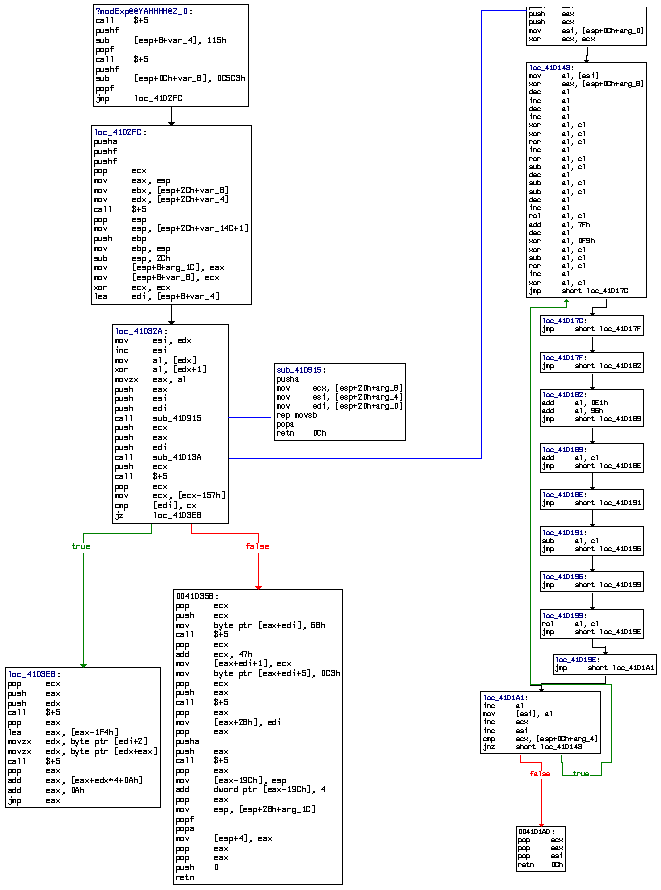
\includegraphics[width=0.7\columnwidth]{./figure/fig_obf_demo_cfg}
\caption{CFG of obfuscated \emph{modexp} function.}
\label{fig_obf_demo_cfg}
\end{figure}





\end{document}
